\documentclass[a4paper,12pt]{article}
\usepackage{graphicx}
\usepackage{caption}
\usepackage{subcaption}

\begin{document}

\begin{figure}
        \centering
        \begin{subfigure}[b]{0.3\textwidth}
                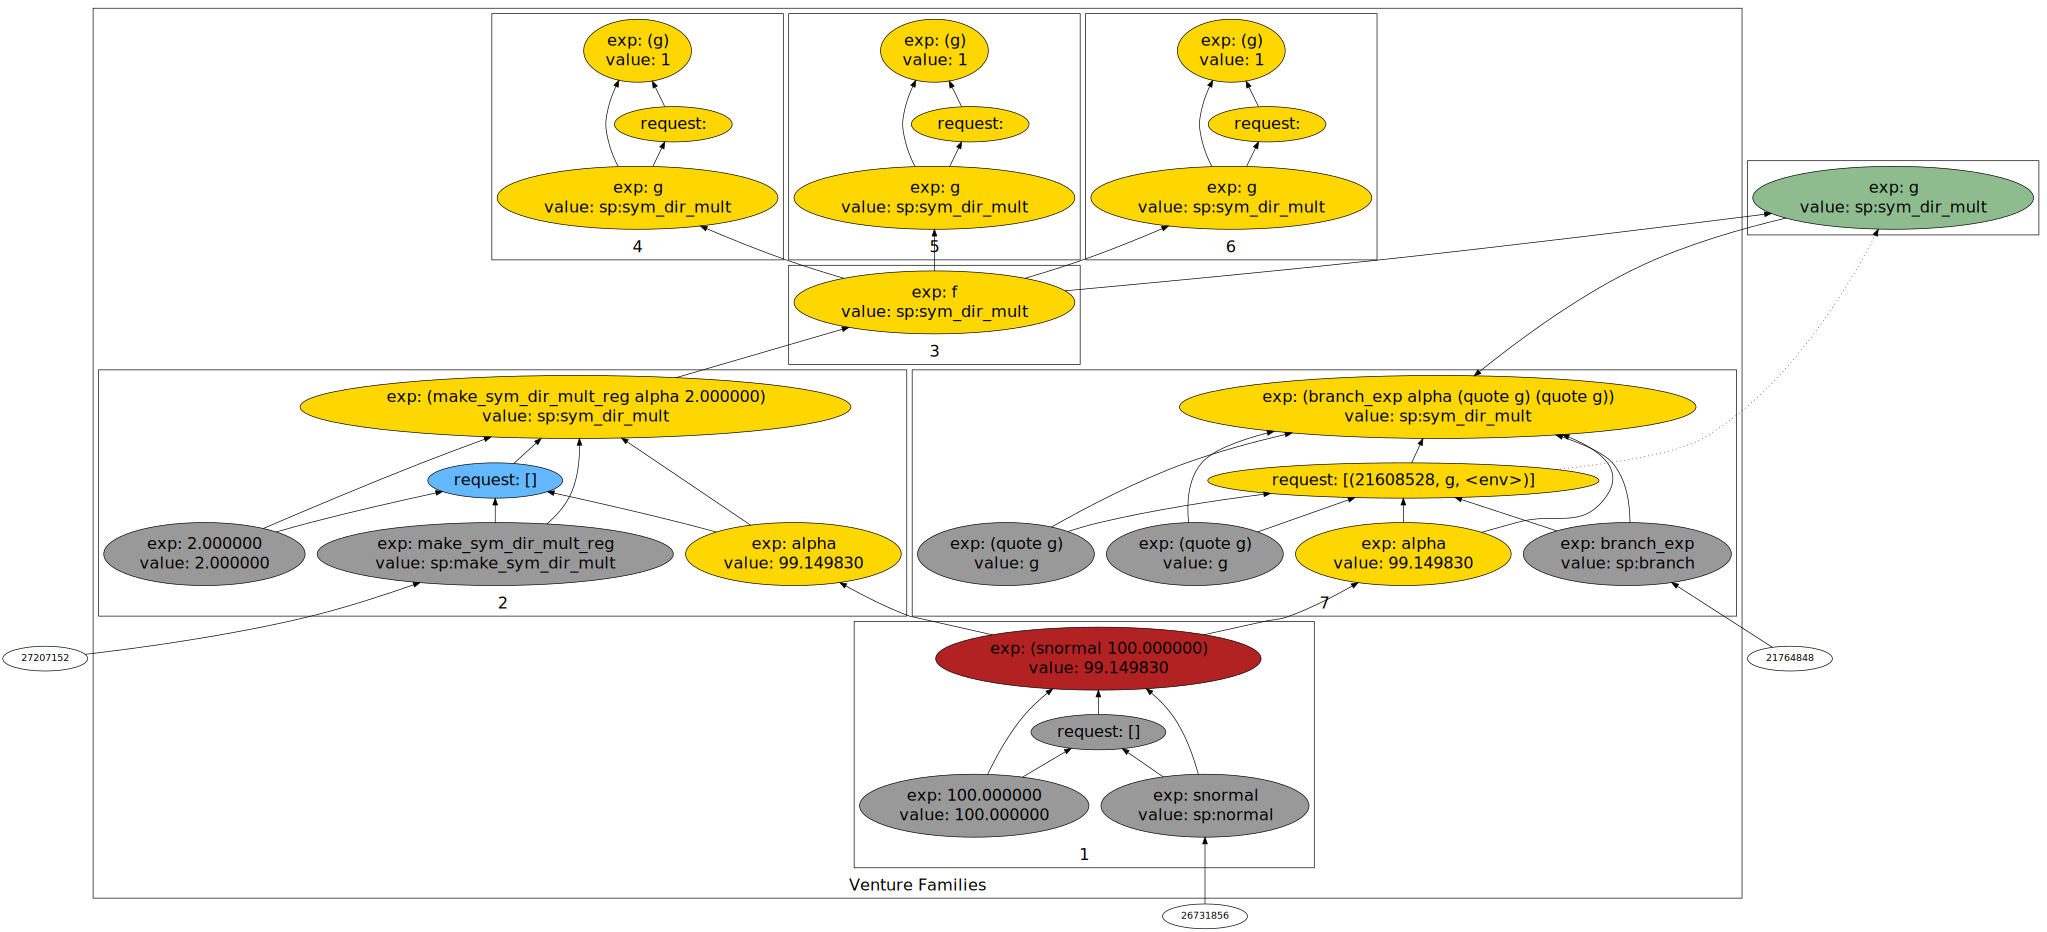
\includegraphics[width=\textwidth]{prior/dot3.pdf}
                \caption{The result of makeSymDirMult is an SP whose applications are exchangeably coupled. Here the result of one application determines whether or not another application is made. Thus the second application is in the brush of the scaffold generated by the first application. If we do not detach the brush first, we may propose to the first application conditioned on  an application that will not exist in the new trace.
}
                \label{fig:gull}
        \end{subfigure}%
 
        ~ %add desired spacing between images, e. g. ~, \quad, \qquad etc.
          %(or a blank line to force the subfigure onto a new line)
        \begin{subfigure}[b]{0.3\textwidth}
                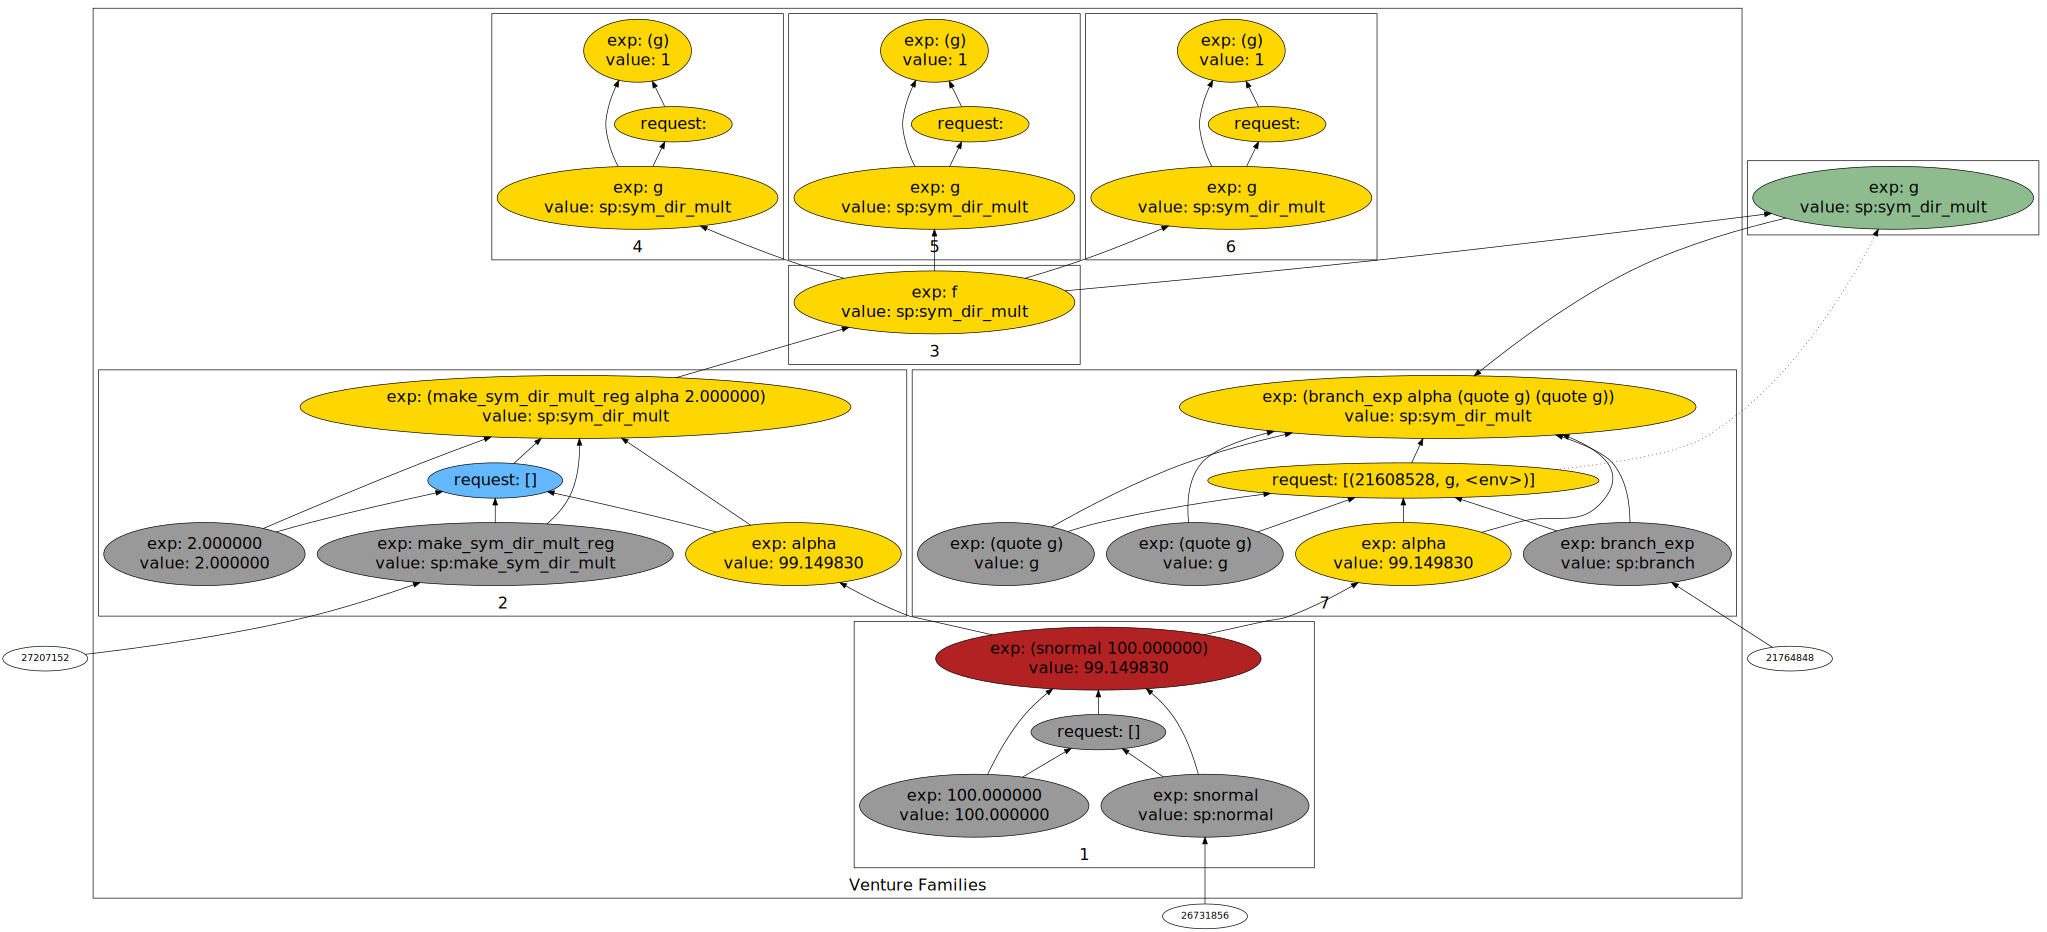
\includegraphics[width=\textwidth]{prior/dot3.pdf}
                \caption{A mouse}
                \label{fig:mouse}
        \end{subfigure}
        \caption{Bleh}

\label{fig:animals}
\end{figure}

\end{document}
